\chapter{CPLEX implementation and performance}

\section{CPLEX}
IBM ILOG CPLEX Optimizer is a solver licensed software, part of the IBM ILOG Optimizer Studio, with high level of efficiency and robustness \cite{IBMILOGCPLEX}. It can resolve a wide variety of problems:
\begin{itemize}
	\item Linear Programming (LP)
	\item Network Flow,
	\item Quadratic Programming (QP),
	\item Quadratically Constrained Programming (QCP),
	\item Mixed Integer Programming (MIP).
\end{itemize}
The interest, for the course purposes, is the LP optimization used to solve the TSP problem. The library written in C language, allow to define and resolve LP models with different heuristics and exact algorithm. The challenge is to implement with a state of the art LP solver the models specified in the chapter \ref{chapter:TSPdescription}, comparing time performance. 

\subsection{Callback}
\subsubsection{Lazy callback}
\subsubsection{Generic callback}



\section{Subtour Elimination}\label{sec:subtour}
The subtour elimination model described above enhance an exponential number of constraint ($ O(2^n) $), therefore it is not practicable to insert all the constraints in the model definition, instead is preferable to resolve the continuous relaxation without subtour elimination and than check if the solution verify the constraints, otherwise add the more violated constraints to the model. Four different version of subtour elimination model has been created:
\begin{enumerate}
	\item \textit{subtour\_iter\_opt}: iterating until there is only one tour, it's applied the optimization step (\texttt{CPX\_mipopt()}) and externally check the subtour constraints and eventually add the violated to the model with \texttt{CPXnewrows()} and \texttt{CPXchgcoef()}. When no constraint is violated the best solution is found.
	\item \textit{subtour\_heur\_iter\_opt}: is equal to the previous one, but in the first iteration the subtour is checked immediately after the first available solution is found (\texttt{CPX\_PARAM\_INTSOLLIM} is set to 1). 
	\item \textit{subtour\_callback\_lazy}: While in the first two method the check is done outside CPLEX, here is used the \texttt{CPXsetlazyconstraintcallbackfunc()}. The lazy constraint, as described in the official CPLEX documentation, are constraints that the user knows are unlikely to be violated, therefore are applied only when necessary, exactly the case of the subtour elimination. The specified function in particular allow to set and modify user-written callback which will be called in two cases: when CPLEX compares an integer-feasible solution to lazy constraints and when the LP at a node is unbounded and when a lazy constraint might cut off the primal ray. Inside the lazy callback, the \texttt{CPXcutcallbackadd()} is used to add the subtour constraints. \\ Note that the lazy callback is not compatible with Dynamic Search (an alternative algorithm to B\&C which is more efficient) which is automatically disabled.
	\item \textit{subtour\_callback\_general}: The \texttt{CPXcallbacksetfunc()} allow to set up a callback specifying the context in which to call that function. In this method is used to apply the lazy constraint with \texttt{CPXcutcallbackadd()} in the \texttt{CPX\_CALLBACKCONTEXT\_CANDIDATE} context. \texttt{CPXcallbacksetfunc()} is compatible with Dynamic Search therefore it is expected to have better performance than \textit{subtour\_callback\_lazy} method.
\end{enumerate} 

\begin{figure}[h]
	\begin{subfigure}{.5\textwidth}
		\centering
		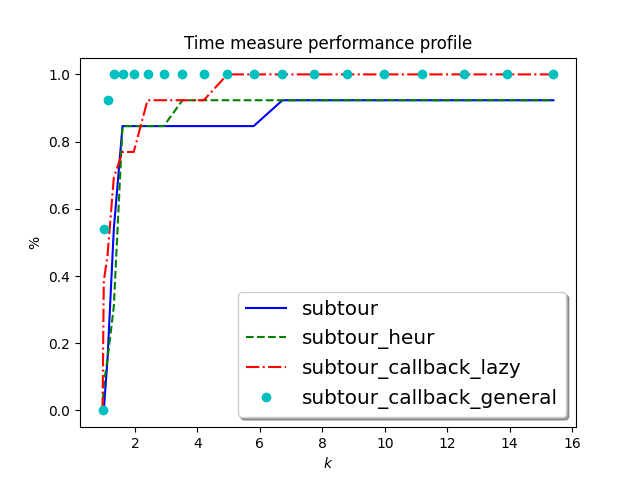
\includegraphics[width=\columnwidth]{../res/Lsubtours_average_time.png}
		\caption{Performance profile of \textit{subtour} models on Data Average}
		\label{fig:res_subtour_av}
	\end{subfigure}
	\begin{subfigure}{.5\textwidth}
	\centering
	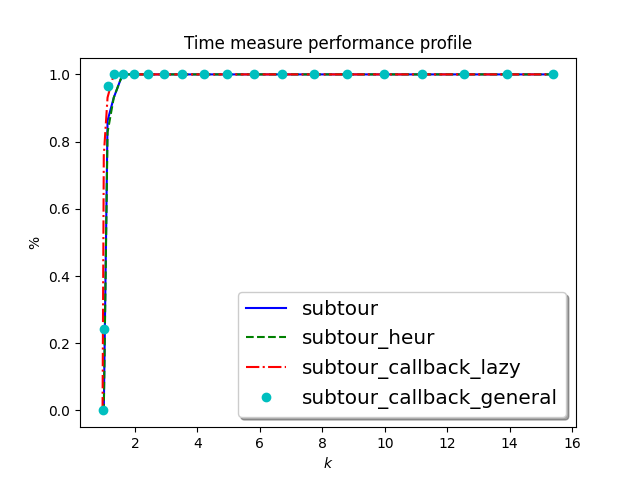
\includegraphics[width=\columnwidth]{../res/Lsubtours_light_time.png}
	\caption{Performance profile of \textit{subtour} models on Data Light}
	\label{fig:res_subtour_li}
	\end{subfigure}
\end{figure}

The performance profile in figure \ref{fig:res_subtour_av} is obtained by executing each subtour method in each Data Average instance for 5 different random seed generator. \\
In this set of instances the \textit{subtour\_callback\_lazy} perform better as expected. In Data Light set no significant evidence is enhance. This is because $ t_{exec} $ is near 10s ($ T_{min} $) and for little differences of $ t_{exec} $ the ratio $ r $ is near 1 (check appendix \ref{sec:performance_meausure} for more details.
Morover it show that in the $ 80\%  $  of the instances the \textit{subtour\_callback\_general} perform better than the other 3 alternatives.\\
\textit{subtour\_heur\_iter\_opt} seems to be faster than \textit{subtour\_iter\_opt} for the discussed optimization. 


\section{Miller Tucker Zemlin}
The number of MTZ constraints is $O(n^2)$ therefore two different models has been proposed to evaluate the callback effectiveness:
\begin{enumerate}
	\item \textit{mtz}: where all the constraints are part of the model definition and added with \texttt{CPXnewrows()} and \texttt{CPXchgcoef()}. 
	\item \textit{mtz\_lazy}: where the MTZ constraints are added as lazy constraints with \texttt{CPXaddlazyconstraints()}, which allow to check the constraints each time an incumbent should be update and to add the violated ones.
\end{enumerate}

performance profile per verificare tra i due quale è il migliore


\section{Flow Chart}


considerazioni sul numero di vincoli e sul problema asimmetrico

dettagli implementativi

performance profile per verificare tra i due quale è il migliore

performance profile con MTZ
